\input{configuration.src}

\addbibresource{./bibliography-collection/lithie.bib}

\title{Trusting Trust Revisited}
\subtitle{Preventing Software Supply Chain Attacks\hfill\\Using Modern Methods}
\institute{Institute of Distributed Systems, Ulm University}
\tag{Seminar}

\author{Florian Sihler}
\email{florian.sihler@uni-ulm.de}
\outro{Ulm, \today}

\date{Februar, 12 2021}

\begin{document}

\section{Motivation}

\begin{frame}{\space}
    \pause{}\begin{layout-imageonly}
    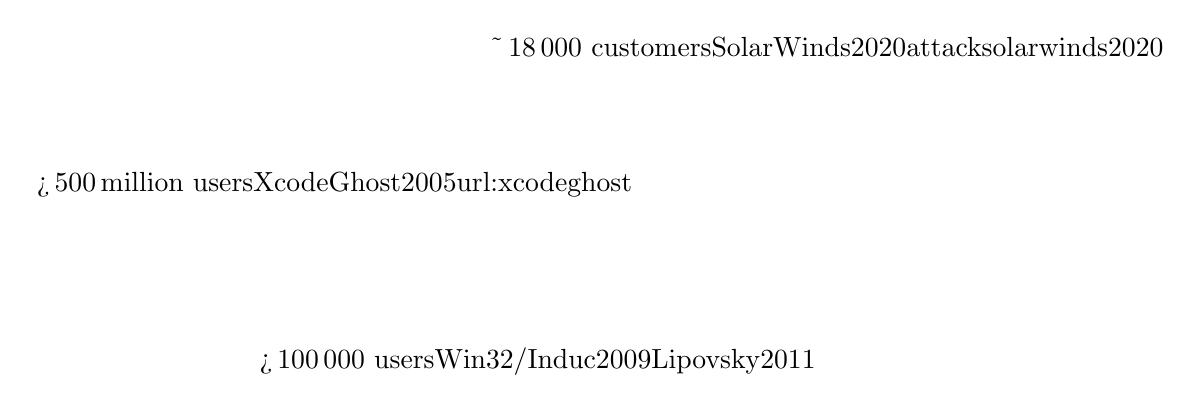
\begin{tikzpicture}
        \node at(0.75,0.25) {\typesetBox{>\,500\,million users}{XcodeGhost}{2005}{url:xcodeghost}};
        \node at(7,2) {\typesetBox{\textasciitilde\,18\,000 customers}{SolarWinds}{2020}{attacksolarwinds2020}};
        \node at(3.33,-2) {\typesetBox{>\,100\,000 users}{Win32/Induc}{2009}{Lipovsky2011}};
    \end{tikzpicture}
\end{layout-imageonly}
\note{\textbf{X Minuten}}
\note[itemize]{
    \item Angriffsmuster Rede von Ken Thompson
    \item >500 mio XcodeGhost
    \item 18\,000 Kunden Solar Winds, auch US-Regierung
    \item 100\,000de Nutzer bei Win32/Induc (Delphi)
}
\end{frame}

\def\tblockfont#1{#1}
\tblocksize=0.95cm
\def\boostrapping{%
\begin{t-diagram}[tborder/.append style={draw=none,fill=lgray,rounded corners=4pt}]
    \begin{scope}[tborder/.append style={fill=btdl@color@secondary}]
        \onslide<2->{\tblock[g]{\tblocksize*8+4*\tblockoffset,2*\tblocksize+2*\tblockoffset}{\SL{}}{\ML{}}{\ML{}}}
    \end{scope}
    \begin{scope}[tborder/.append style={densely dashed}]
    \onslide<3->{\tblock[b]{2*\tblocksize+\tblockoffset,-\tblocksize-\tblockoffset}{T}{\ML{}}{\ML{}}}
        \onslide<5->{\tblock[c]{\tblocksize*4+\tblockoffset*2,0}{\SL0}{\ML{}}{\ML{}}}
        \onslide<7->{\tblock[f]{\tblocksize*6+3*\tblockoffset,\tblocksize+\tblockoffset}{\SL1}{\ML{}}{\ML{}}}
    \end{scope}
    \onslide<4->{\tblock[a]{0,0}{\SL0}{\ML{}}{T}}
    \onslide<6->{\tblock[d]{\tblocksize*2+\tblockoffset,\tblocksize+\tblockoffset}{\SL1}{\ML{}}{\SL0}}
    \onslide<8->{\tblock[e]{\tblocksize*4+2*\tblockoffset,2*\tblocksize+2*\tblockoffset}{\SL{}}{\ML{}}{\SL1}}
\end{t-diagram}
}

\section{The Attack}
\SidebarCite{book:mckeemanCompilerGenerator}
\SidebarCite{Thompson1984}
\newsavebox\bootstrapbox
\savebox\bootstrapbox{\def\onslide<#1>#2{#2}\boostrapping}

\makeatletter
\begin{frame}[fragile]{The Attack}
\begin{layout-imageonly}
    \only<1-8|handout:0>{\begin{center}\scalebox{0.9}{\boostrapping}\end{center}}
    \only<9->{%
    \begin{tikzpicture}
        \node[scale=0.6,right] (bootstrap) at (0,0) {\usebox{\bootstrapbox}};
        \begin{scope}[shift=(bootstrap.east),xshift=1.85cm,yshift=-0.69cm]
        \onslide<12->{\node[bc] (0) at (0,1.4) {\faFileText};}
        \onslide<13->{
            \node[bc=lgray] (1) at (0,0) {\faFile\llap{\color{lgray}\tiny\faCogs\;}};
            \draw[-Kite,ultra thick,btdl@color@secondary] (0) -- (1);
        }
        \onslide<14->{
            \node[bc] (2) at (2,0) {\cfl{btdl@color@secondary}};
            \draw[-Kite,ultra thick,btdl@color@secondary] (1) -- (2);
        }
        \onslide<15->{
            \node[bc=lgray] (3) at (2,1.4) {\faFileText};
            \draw[-Kite,ultra thick,lgray] (3) -- (2);
        }

        \onslide<16->{
            \node[bc] (4) at (4,0) {\cfl{btdl@color@secondary}};
            \draw[-Kite,ultra thick,btdl@color@secondary] (2) -- (4);
        }


        % \node[bc] (2) at (4,0) {\cfl{btdl@color@secondary}}};
        \end{scope}
        \node at(0,-3.5) {};
    \end{tikzpicture}
    }%
\begin{onlyenv}<9->
\strut~\vspace*{-7em}\\
\hspace*{.265\linewidth}\begin{minipage}[b]{0.75\linewidth}
\lstfs{8}\begin{plaincpp}[morekeywords={[1]{if,contains}},morekeywords={[4]{source}}]
!*\onslide<11->*!inject = 'inject = %c%s%c;
if source contains "compile()":
  prepend("compile()", inject % 34, inject, 34)'

if source contains "compile()":
  prepend("compile()", inject % 34, inject, 34)

!*\onslide<10->*!compile();
\end{plaincpp}
% !*\onslide<10->*!if source contains "if(check(pw))":
% !*\onslide<10->*!  replace(line, "check", "\"a\" == ");
\end{minipage}%
\end{onlyenv}% fake slidecounter thinking max
\only<9-10>{}%
\end{layout-imageonly}
\note{\textbf{Y Minuten}}
\note[itemize]{
    \item Zuerst: Bootstrapping (Go-Compiler seit 1.5)
    \item Wir vereinfachen einmal mit 'compile'
    \item Einbau von Quine
    \item Einfügen des immer selben Codes (lässts ich erweitern)
    \item Infiziert nachfolger
}
\end{frame}
\SidebarReset

\section{Diverse Double Compiling}
% \SidebarCite{pdf:ddc}
\nocite{pdf:ddc}
\begin{frame}{Diverse Double Compiling}
    \begin{layout-imageonly}
        \begin{tikzpicture}[bc/.default={lgray}]
            \onslide<2->{\node[bc] (0) at (0,1.4) {\faFileText};}
            \onslide<3->{\node[bc] (1) at (-1.25,0) {\!\faLaptop};
            \node[bc] (2) at ( 0,0) {\!\faLaptop};
            \node[bc] (3) at ( 1.25,0) {\!\faLaptop};

            \draw[-Kite,ultra thick,lgray] (0) -- (1);
            \draw[-Kite,ultra thick,lgray] (0) -- (2);
            \draw[-Kite,ultra thick,lgray] (0) -- (3);}

            \onslide<4->{\node[bc=lgray] (a1) at (-1.25,-1.4) {\cfl{lgray}};
            \node[bc=lgray] (a2) at ( 0,-1.4) {\cfl{lgray}};
            \node[bc=lgray] (a3) at ( 1.25,-1.4) {\cfl{lgray}};

            \draw[-Kite,ultra thick,lgray] (1) -- (a1);
            \draw[-Kite,ultra thick,lgray] (2) -- (a2);
            \draw[-Kite,ultra thick,lgray] (3) -- (a3);}

            \onslide<5->{\path (a1) -- (a2) node[btdl@color@primary,pos=0.5] {$=$};
            \path (a2) -- (a3) node[btdl@color@primary,pos=0.5] {$=$};}
            \onslide<2->{\node[below=.15cm] at (current bounding box.south) {Reproducible};}

            \begin{scope}[xshift=5.5cm]
                \onslide<6->{\node[bc] (0) at (0,1.4) {\faFileText};
                \node[left=0.5cm] at(0.west) {1.}; \tagS{0}{A}}
                \onslide<7->{\node[bc] (1) at (2,1.4) {\!\faCogs};
                \draw[-Kite,ultra thick,lgray] (0) -- (1); \tagN{1}{A}}
                \onslide<8->{\node[bc] (2) at (4,1.4) {\cfl{lgray}};
                \draw[-Kite,ultra thick,lgray] (1) -- (2); \tagS{2}{A}}
                \begin{pgfonlayer}{background}
                    \onslide<9->{\draw[btdl@color@primary,ultra thick] (1) to[bend left=42,edge node={node[circle,fill=white,inner sep=2pt] {$=$}}] (2);}
                \end{pgfonlayer}


                \onslide<10->{\node[bc] (3) at (0,0) {\faFileText};
                \tagS{3}{A}
                \node[left=0.5cm] at(3.west) {2.};}
                \onslide<11->{\node[bc] (4) at (2,0) {\!\faCogs};
                \tagN{4}{B}\draw[-Kite,ultra thick,lgray] (3) -- (4);}
                \onslide<12->{\node[bc] (5) at (2,-1.4) {\cfl{lgray}};
                \tagS{5}{A}
                \draw[-Kite,ultra thick,lgray] (4) -- (5);}

                \onslide<13->{\node[bc] (6) at (0,-1.4) {\faFileText};
                \tagS{6}{A}
                \draw[-Kite,ultra thick,lgray] (6) -- (5);}

                \onslide<14->{\node[bc] (7) at (4,-1.4) {\cfl{lgray}};
                \tagS{7}{A}
                \draw[-Kite,ultra thick,lgray] (5) -- (7);}

                \begin{pgfonlayer}{background}
                    \onslide<15->{\draw[btdl@color@primary,ultra thick] (2) to[bend left=42,edge node={node[circle,fill=white,inner sep=2pt] {$=$}}] (7);}
                \end{pgfonlayer}
            \end{scope}

        \end{tikzpicture}
    \end{layout-imageonly}
\end{frame}
% \SidebarReset

\section{CHAINIAC}

\begin{frame}{CHAINIAC}
    Hello \cite{Nikitin2017}!
\end{frame}

\section{Conclusion}

\begin{frame}{Conclusion}
    Hello
\end{frame}


\pdfbookmark[0]{Endfolie -- Quellen}{endfolie}%
\end{document}
